% Title:
% 	Presentation template
% ----------------------
% Description:
% 	A clean, sans-serif presentation template.
%   This presentation uses custom fonts. You need to compile with xelatex,
%   and download Open Sans and Ubuntu Mono from:
%	
%	- https://www.fontsquirrel.com/fonts/open-sans
%	- https://www.fontsquirrel.com/fonts/ubuntu-mono
%
% Creator: Tommy Odland

% -------------------------------------------------------------------------
% Setup
% -------------------------------------------------------------------------
% Options for aspectratio: 1610, 149, 54, 43 and 32, 169
\documentclass[12pt, aspectratio=149]{beamer}
\usepackage[utf8]{inputenc}
\usepackage[english]{babel}% Alternatives: 'norsk', 'english'
\usepackage[expansion=false]{microtype}% Fixes to make typography better
\usecolortheme{beaver} % Decent options: beaver, rose, crane
%\useoutertheme{split}
%\useoutertheme[footline=authortitle]{miniframes}
\usepackage{listings}% To include source-code
\usepackage{booktabs}% Professional tables
\usepackage{multirow}
\usepackage{xcolor}

\definecolor{links}{HTML}{2A1B81}
\hypersetup{colorlinks,linkcolor=,urlcolor=links}

% https://tex.stackexchange.com/questions/159667/including-python-code-in-beamer
% https://ftp.eq.uc.pt/software/TeX/macros/latex/contrib/minted/minted.pdf
\usepackage{minted}

% Title information common to every file
\institute{Equinor}
\date{Edited: \today}
\author{Tommy Odland \and Knut Utne Hollund}

% -------------------------------------------------------------------------
% Package imports
% -------------------------------------------------------------------------
\usepackage{etoolbox}
\usepackage{graphicx}
\usepackage{tikz}
\usepackage{amsmath,amsthm,amsfonts,amssymb,mathtools, bm}
\usepackage{hyperref}
\usepackage{listings}
\usepackage[sharp]{easylist}
\usepackage{multicol}
\usepackage{tikz-cd}

\usepackage[absolute,overlay]{textpos}
\setbeamertemplate{footline}[frame number]  
\usepackage{graphbox}

\newcommand{\norm}[1]{\left\lVert#1\right\rVert}

\setbeamertemplate{footline}{%
%	\includegraphics[align=c, height=0.5cm]{figs/sonat_logo_color.png}%
	\hfill%
	\usebeamercolor[fg]{page number in head/foot}%
%	\usebeamerfont{page number in head/foot}%
%	\insertframenumber\,/\,\inserttotalframenumber\kern1em%
}

% Set the math fonts - should be set before the others fonts, not sure why
\usepackage{sansmath} % Enables turning on sans-serif math mode
% \sansmath % Enable sans-serif math for rest of document

% Set fonts to Open Sans and Ubuntu mono
\usefonttheme{professionalfonts}
\usepackage{fontspec}
%\setmainfont{Open Sans}
%\setsansfont{Open Sans}
\setmonofont{Ubuntu Mono}
%\usefonttheme{serif}

\usepackage[mathrm=sym]{unicode-math}
\setmathfont{Fira Math}

%gets rid of bottom navigation symbols
\setbeamertemplate{navigation symbols}{}

% Set up colors to be used
\definecolor{titlecolor}{RGB}{128,54,63}
\definecolor{bggray}{RGB}{242,242,242}
\definecolor{bggraydark}{RGB}{217,217,217}

% Change the default colors
\setbeamercolor*{title}{bg=bggray,fg=titlecolor}
\AtBeginEnvironment{theorem}{%
	\setbeamercolor{block title}{fg=titlecolor, bg=bggraydark}
	\setbeamercolor{block body}{fg=black,bg=bggray}
}
\AtBeginEnvironment{proof}{%
	\setbeamercolor{block title}{fg=titlecolor, bg=bggraydark}
	\setbeamercolor{block body}{fg=black,bg=bggray}
}
\AtBeginEnvironment{example}{%
	\setbeamercolor{block title example}{bg=bggraydark}
	\setbeamercolor{block body example}{fg=black,bg=bggray}
}
\AtBeginEnvironment{definition}{%
	\setbeamercolor{block title}{bg=bggraydark}
	\setbeamercolor{block body}{fg=black,bg=bggray}
}

\setbeamercolor{block title example}{bg=bggraydark}
\setbeamercolor{block body example}{fg=black,bg=bggray}
\setbeamercolor{block title}{fg=titlecolor, bg=bggraydark}
\setbeamercolor{block body}{fg=black,bg=bggray}

\setbeamercolor{frametitle}{fg=titlecolor,bg=bggray}
\setbeamercolor{section in head/foot}{bg=black}
\setbeamercolor{author in head/foot}{bg=black}
\setbeamercolor{date in head/foot}{fg=titlecolor}

% Spacing for lists
\newcommand{\listSpace}{0.2em}

% Theorems, equations, definitions setup
\theoremstyle{plain}

% Slides for sections
\AtBeginSection[]{
	\begin{frame}
		\vfill
		\centering
		\begin{beamercolorbox}[sep=8pt,center,shadow=false,rounded=false]{title}
			\usebeamerfont{title}\insertsectionhead\par%
		\end{beamercolorbox}
		\vfill
	\end{frame}
}

% Title information
\title{Wanna see my collection of random numbers?}
\subtitle{Course overview}

% -------------------------------------------------------------------------
% Document start
% -------------------------------------------------------------------------
\begin{document}

\begin{frame}{}
	\begin{center}
			\vfill
	{\huge Wanna see my collection of random numbers?}
	\vfill
	{\large A crash course in computational statistics}
	\vfill

	\vfill
	{\large  \texttt{@tommyod} \texttt{@KnutUH}}
	\vfill
	{\small \href{https://github.com/tommyod/rng}{https://github.com/tommyod/rng}}

	\vfill
	\today 
	% September 15, 2023
	\vfill
	\end{center}
\end{frame}

\begin{frame}[fragile]{Agenda}
	
	\begin{easylist}[itemize]
		# \textbf{Statistical Concepts} 
		# \textbf{Monte Carlo Simulation}
		# \textbf{Resampling}
		# \textbf{Stochastic Search} 
		# \textbf{Bayesian Statistics} 
	\end{easylist}
	\hspace{4em}

	In this presentation, we'll see that programming and random number generation make life much easier!
\end{frame}


% ==================================================================
% ==================================================================
% ==================================================================
\section{Statistical Concepts}

\begin{frame}[fragile]{Probability}

	A probability $P$ is a function defined on events in a sample space $S$, that satisfies:
	\begin{align*}
		& 0 \leq P(A) \leq 1  & & \text{for all events $A$} \\
		& P(S) = 1 & & \\
		& P(A_{1} \cup A_{2} \cup \ldots) & \hspace*{1em} & \text{for all disjoint events $A_{1}, A_{2}, \ldots$}	
	\end{align*}  
	
\end{frame}


\begin{frame}[fragile]{Human height - distributions}
    \begin{center}
     \begin{figure}
     	\centering
     	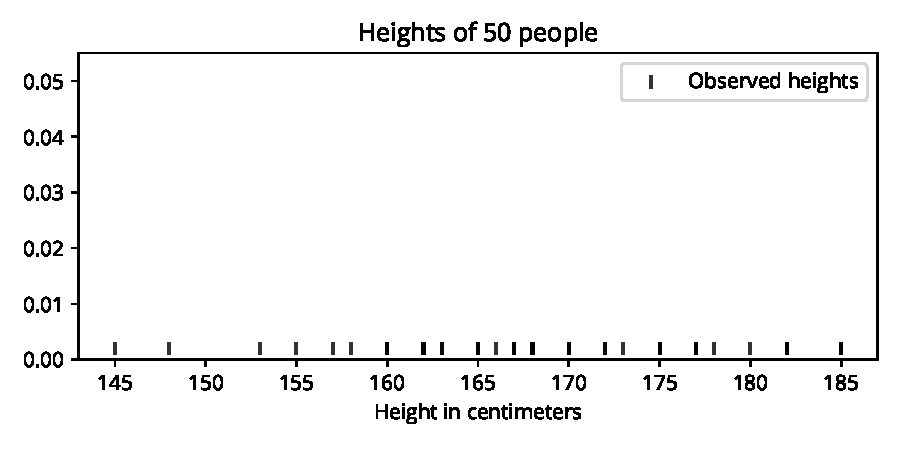
\includegraphics[width=0.99\linewidth]{figures/heights_1}
     \end{figure}
     \end{center}
\end{frame}

\begin{frame}[fragile]{Human height - distributions}
    \begin{center}
     \begin{figure}
     	\centering
     	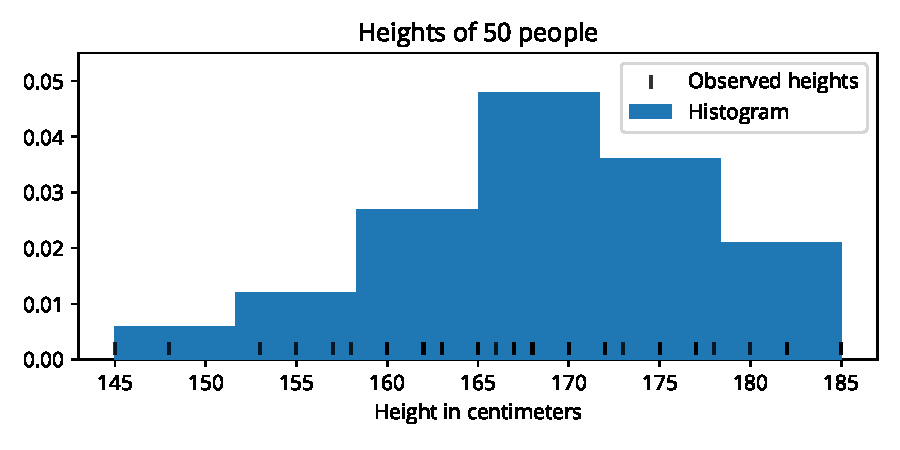
\includegraphics[width=0.99\linewidth]{figures/heights_2}
     \end{figure}
     \end{center}
\end{frame}

\begin{frame}[fragile]{Human height - distributions}
    \begin{center}
     \begin{figure}
     	\centering
     	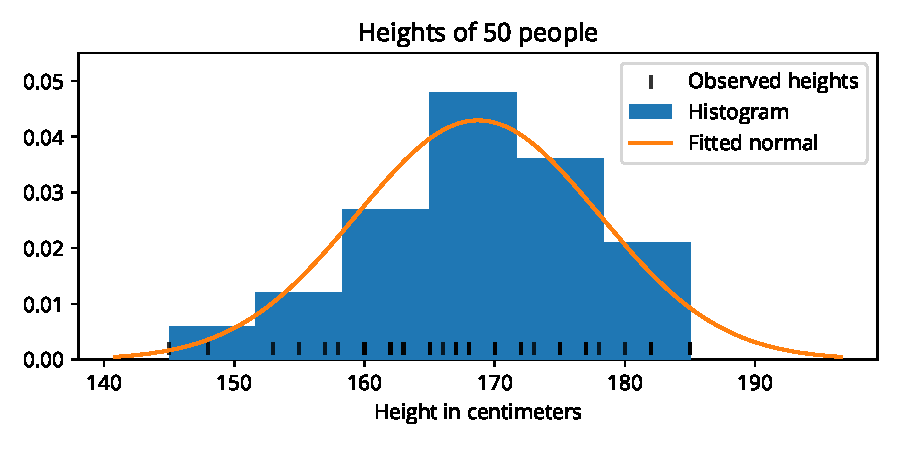
\includegraphics[width=0.99\linewidth]{figures/heights_3}
     \end{figure}
     Mean value: $168.7$ \hspace*{4em} Standard deviation: $9.3$
     \end{center}
\end{frame}

\begin{frame}[fragile]{Human height - cumulative distributions}
    \begin{center}
     \begin{figure}
     	\centering
     	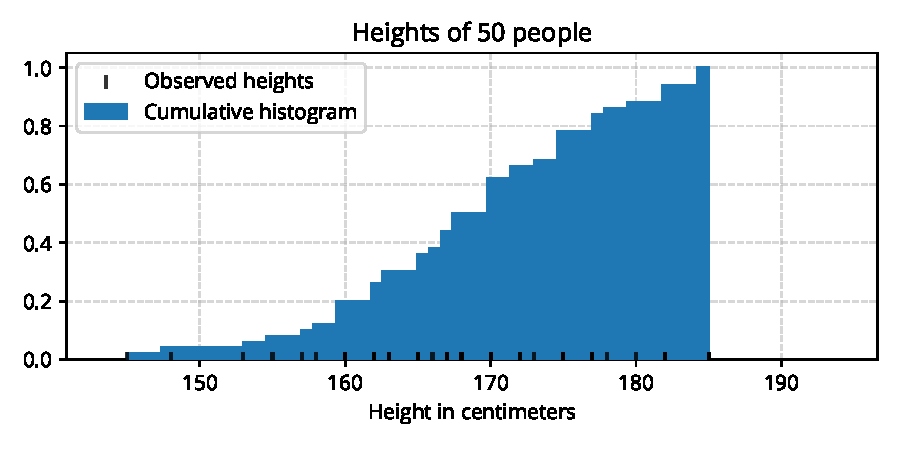
\includegraphics[width=0.99\linewidth]{figures/heights_cumulative_2}
     \end{figure}
     Empirical percentiles:\\$P10 = 157.9$,\hspace*{1em} $P50 = 169$,\hspace*{1em} $P90 = 182$
     \end{center}
\end{frame}

\begin{frame}[fragile]{Human height - cumulative distributions}
    \begin{center}
     \begin{figure}
     	\centering
     	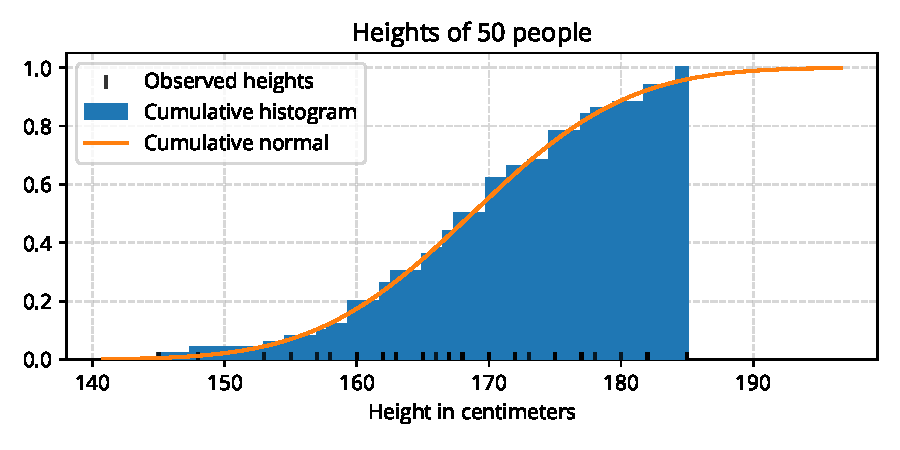
\includegraphics[width=0.99\linewidth]{figures/heights_cumulative_3}
     \end{figure}
     Normal percentiles:\\$P10 = 156.8$,\hspace*{1em} $P50 = 168.7$,\hspace*{1em} $P90 = 180.6$
     \end{center}
\end{frame}

\begin{frame}[fragile]{Random Variables and Probability Distributions}
	\begin{figure}
		\centering
		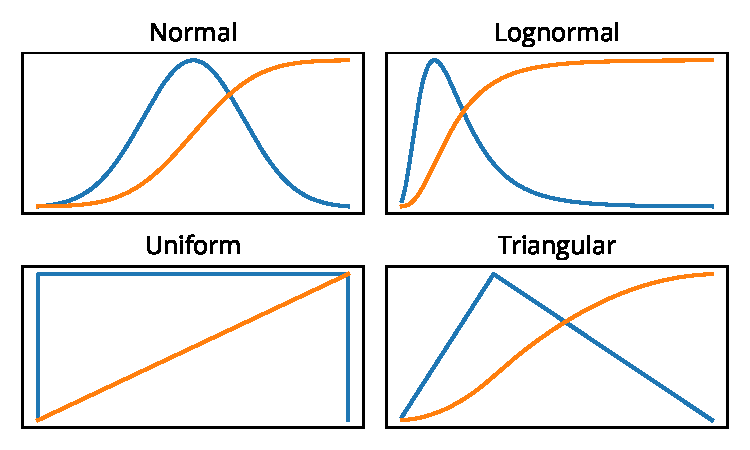
\includegraphics[width=0.99\linewidth]{figures/pdfs_cdfs_v2}
	\end{figure}
\end{frame}



\begin{frame}[fragile]{Mean, median and mode}
	\begin{columns}
		\begin{column}{0.5\textwidth}
			\begin{easylist}[itemize]
			# Expected value (mean): 
			## weighted average of possible outcomes. Also
			center of gravity of the density

			# Median (P50): 
			## same area above and below
	
			# Most likely value (mode): 
			## maximum of the PDF

			# In a symmetric distribution all three coincide
			\end{easylist}
		\end{column}
		\begin{column}{0.5\textwidth}
			\begin{figure}
				%\centering
				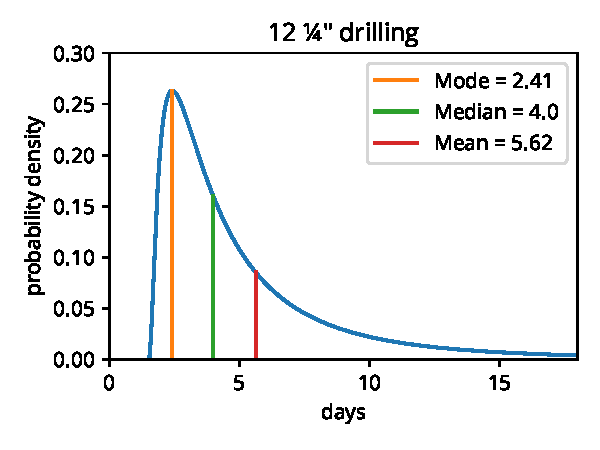
\includegraphics[width=0.99\linewidth]{figures/lognorm_pdf}
			\end{figure}
		\end{column}
	\end{columns}
	\end{frame}
	

\begin{frame}[fragile]{Calculations with distributions}
	What is the distribution of total time ($Z$) for two independent tasks ($X + Y$), when the distribution for each task is known?
    \begin{center}
     \begin{figure}
     	\centering
     	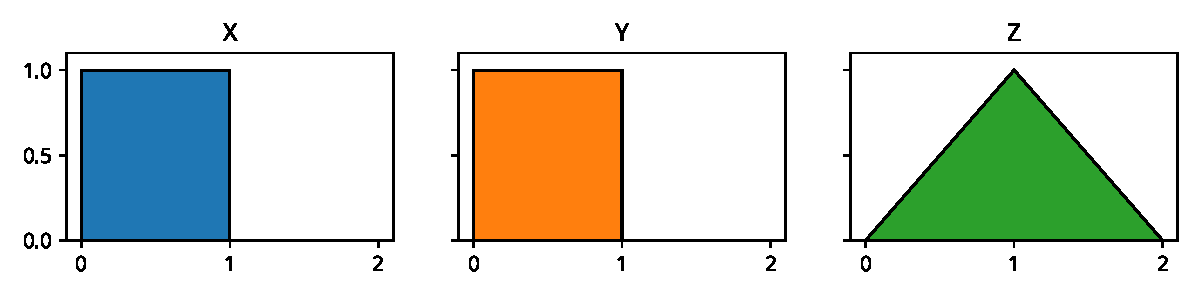
\includegraphics[width=0.99\linewidth]{figures/add_uniform}
     \end{figure}
     \end{center}
	 \begin{flalign*}
     &\hspace*{1em} P10_X = 1.1 \hspace*{4em} P10_Y = 1.1 \hspace*{4em}  P10_Z = ? \\
	 &\hspace*{1em} E(X) = 1.5  \hspace*{4.2em} E(Y) = 1.5  \hspace*{4.3em}  E(Z)= ? \\
     &\hspace*{1em} P90_X = 1.9 \hspace*{4em} P90_Y = 1.9 \hspace*{4em}  P90_Z = ? \\
	\end{flalign*}
\end{frame}

\begin{frame}[fragile]{Calculations with distributions}
	What is the distribution of total time ($Z$) for two independent tasks ($X + Y$), when the distribution for each task is known?
    \begin{center}
     \begin{figure}
     	\centering
     	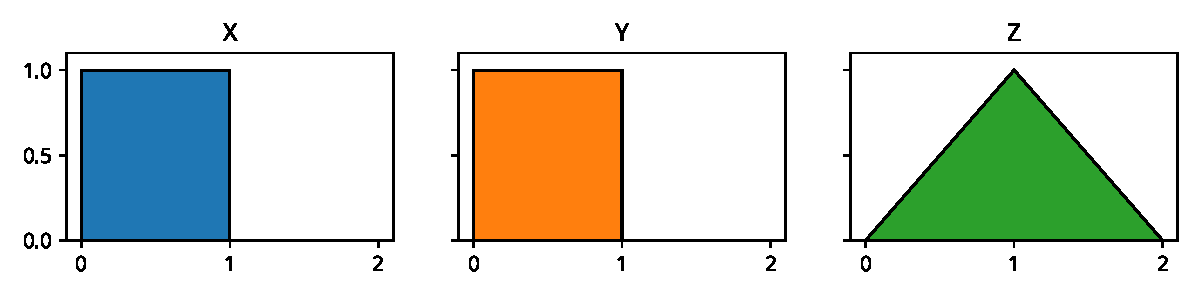
\includegraphics[width=0.99\linewidth]{figures/add_uniform}
     \end{figure}
     \end{center}
	 \begin{flalign*}
     	&\hspace*{1em} P10_X = 1.1 \hspace*{4em} P10_Y = 1.1 \hspace*{4em}  P10_Z = 2.45 \\
	 	&\hspace*{1em} E(X) = 1.5  \hspace*{4.2em} E(Y) = 1.5  \hspace*{4.3em}  E(Z)= 3 \\
     	&\hspace*{1em} P90_X = 1.9 \hspace*{4em} P90_Y = 1.9 \hspace*{4em}  P90_Z = 3.55 \\
	\end{flalign*}
\end{frame}

\begin{frame}[fragile]{Computational rules}
	Mean (expected value):
	\begin{flalign*}
		& E(a + bX) = a + bE(X) \\
		& E(X + Y) = E(X) + E(Y) \\
		& E(XY) = E(X)E(Y) \hspace*{1em} \text{if $X$ and $Y$ are independent} \\
		& E(XY) \neq E(X)E(Y) \hspace*{1em} \text{if $X$ and $Y$ are dependent}
	\end{flalign*}

	Variance:
	\begin{align*}
		& \operatorname{Var}(a + bX) = b^{2}\operatorname{Var}(X) \\
		& \operatorname{Var}(X + Y) = \operatorname{Var}(X) + \operatorname{Var}(Y) + 2\operatorname{Cov}(X,Y) \\
		& \operatorname{Var}(X - Y) = \operatorname{Var}(X) + \operatorname{Var}(Y) - 2\operatorname{Cov}(X,Y) \\
	\end{align*}

	\onslide<2->{
		\begin{tikzpicture}[remember picture, overlay]
			\draw[line width=8pt, red] (current page.north west) -- (current page.south east);
			\draw[line width=8pt, red] (current page.north east) -- (current page.south west);
			% \draw[fill, white](current page.center, current page.center) ;	
		\end{tikzpicture}
	}
\end{frame}

\begin{frame}[fragile]{Statistical Concepts}
	\begin{easylist}[itemize]
		# To handle uncertainty in a consistent way, knowledge about probability, PDFs or CDFs are needed
		# Four common probability distributions are:
		\begin{columns}
		\begin{column}{0.5\textwidth}
			\begin{easylist}[itemize]
				## uniform
				## triangular
			\end{easylist}
		\end{column}
		\begin{column}{0.5\textwidth}  %%<--- here
			\begin{easylist}[itemize]
				## normal
				## lognormal
			\end{easylist}
		\end{column}
		\end{columns}
		# Important properties: the mean (expected value), P10, P50 (median), P90
		# Theoretical rules for manipulating probabilities are difficult
	\end{easylist}
\end{frame}
	


% ==================================================================
% ==================================================================
% ==================================================================
\section{Monte Carlo Simulation}

\begin{frame}[fragile]{Probability Density Functions (PDFs)}
	\begin{columns}
	\begin{column}{0.5\textwidth}
		\begin{center}
		 \begin{figure}
			 \centering
			 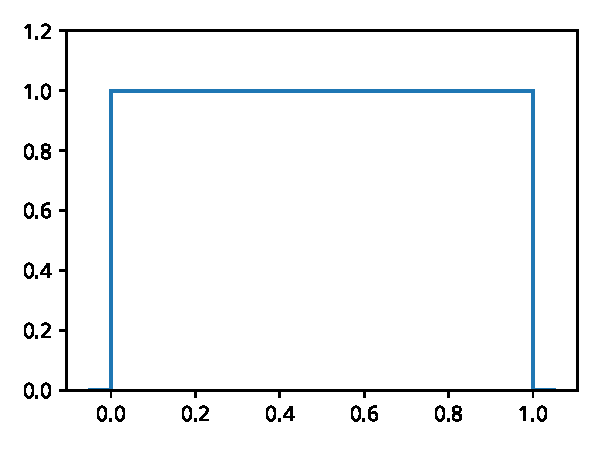
\includegraphics[width=0.99\linewidth]{figures/uniform}
		 \end{figure}
		 \begin{minted}{pycon}
>>> import random
>>> random.random()
0.9757805031464292
		 \end{minted}
		 \end{center}
	\end{column}
	\begin{column}{0.5\textwidth}  %%<--- here
		\begin{center}
		 \begin{figure}
			 \centering
			 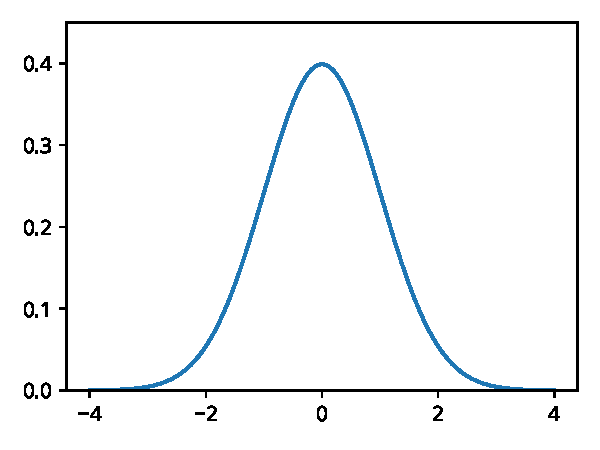
\includegraphics[width=0.99\linewidth]{figures/normal}
		 \end{figure}
		  \begin{minted}{pycon}
>>> import random
>>> random.gauss(0, 1)
-0.19223758016631237
		  \end{minted}
		 \end{center}
	\end{column}
	\end{columns}
	\end{frame}


\begin{frame}[fragile]{Sampling PDFs}
	\begin{columns}
	\begin{column}{0.5\textwidth}
		\begin{center}
		 \begin{figure}
			 \centering
			 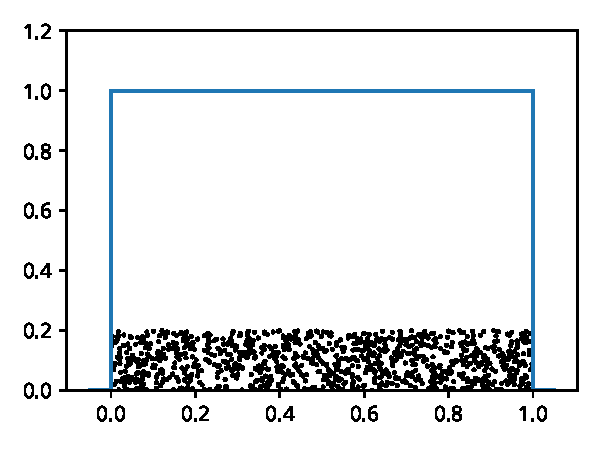
\includegraphics[width=0.99\linewidth]{figures/uniform_samples}
		 \end{figure}
		 \begin{minted}{pycon}
>>> import random
>>> random.random()
0.9757805031464292
		 \end{minted}
		 \end{center}
	\end{column}
	\begin{column}{0.5\textwidth}  %%<--- here
		\begin{center}
		 \begin{figure}
			 \centering
			 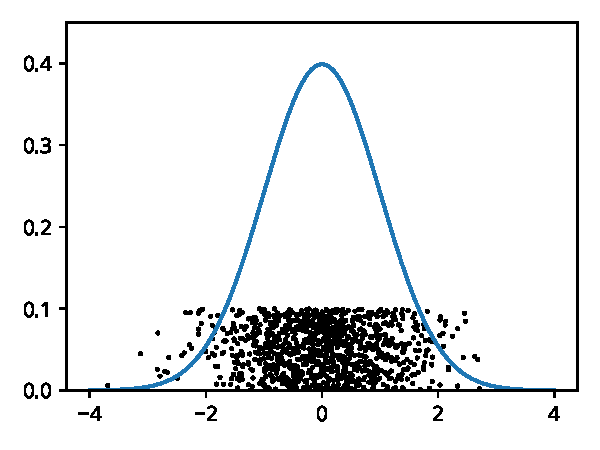
\includegraphics[width=0.99\linewidth]{figures/normal_samples}
		 \end{figure}
		  \begin{minted}{pycon}
>>> import random
>>> random.gauss(0, 1)
-0.19223758016631237
		  \end{minted}
		 \end{center}
	\end{column}
	\end{columns}
\end{frame}
	
\begin{frame}[fragile]{Using samples to generate histograms}
\begin{columns}
\begin{column}{0.5\textwidth}
	\begin{center}
 \begin{figure}
	 \centering
	 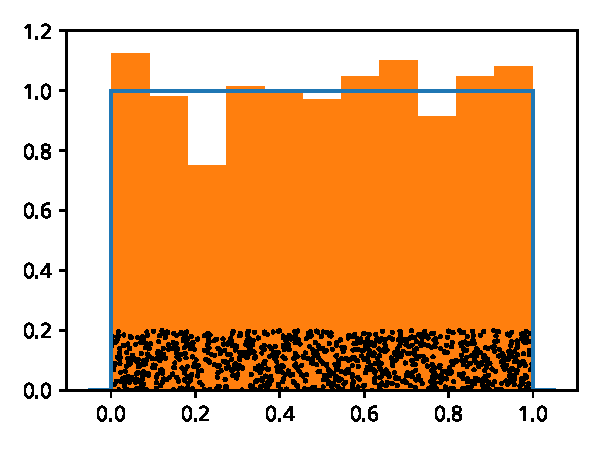
\includegraphics[width=0.99\linewidth]{figures/uniform_samples_hist}
 \end{figure}
 \begin{minted}{pycon}
>>> import random
>>> random.random()
0.9757805031464292
 \end{minted}
 \end{center}
\end{column}
\begin{column}{0.5\textwidth}  %%<--- here
	\begin{center}
 \begin{figure}
	 \centering
	 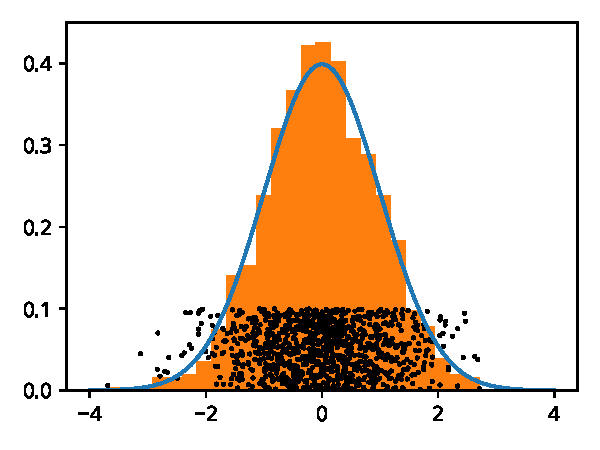
\includegraphics[width=0.99\linewidth]{figures/normal_samples_hist}
 \end{figure}
 \begin{minted}{pycon}
>>> import random
>>> random.gauss(0, 1)
-0.19223758016631237
 \end{minted}
 \end{center}
\end{column}
\end{columns}
\end{frame}

\begin{frame}{Monte Carlo Simulation}
	\begin{figure}
		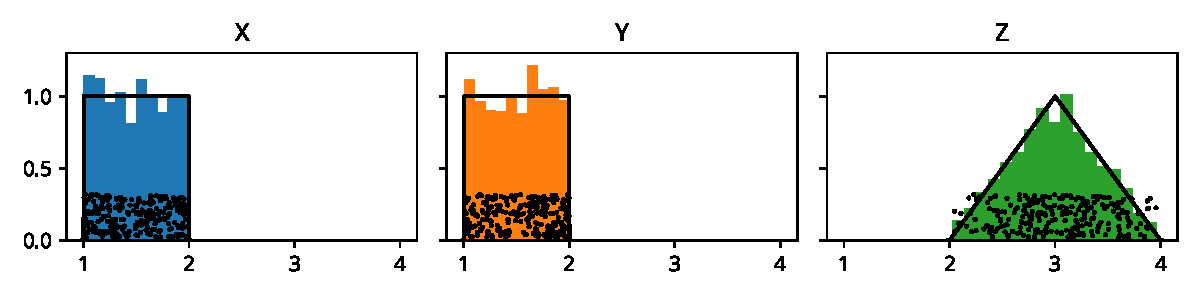
\includegraphics[width=0.99\linewidth]{figures/add_uniform_samples}
	\end{figure}
	% would be cool to get this table generated from our code
	
	% it ain't pretty, but it works
%	\begin{tabular}{lclcl}
%	$P10_x = 1.095$ &\hspace*{2em}& $P10_y = 1.108$ &\hspace*{2em}& $ P10_z = 2.450$ \\
%	$\overline{x} = 1.491$ &\hspace*{2em}& $\overline{y} = 1.517$ &\hspace*{2em}& $ \overline{z}= 3.008$ \\
%	$P90_x = 1.900$ &\hspace*{2em}& $P90_y = 1.890$ &\hspace*{2em}& $ P90_z = 3.594$ \\
%	\end{tabular}

	\begin{center}
	Recall the sum $Z = f(X, Y) = X + Y$ of times for two different tasks.
	\end{center}
	
	
	\begin{flalign*}
		&\hspace*{1em} P10_x = 1.095 \hspace*{4em} P10_y = 1.108 \hspace*{4em}  P10_z = 2.427 \\
		&\hspace*{1em} \overline{x} = 1.491 \hspace*{5.5em}  \overline{y} = 1.517 \hspace*{5.9em}   \overline{z}= 3.008 \\
		&\hspace*{1em} P90_x = 1.900 \hspace*{4em} P90_y = 1.890 \hspace*{4em}  P90_z = 3.569 \\
   \end{flalign*}
\end{frame}

\begin{frame}[fragile]{Cannonball}
\vspace*{-1em}
\begin{center}
 \begin{figure}
    	\centering
    	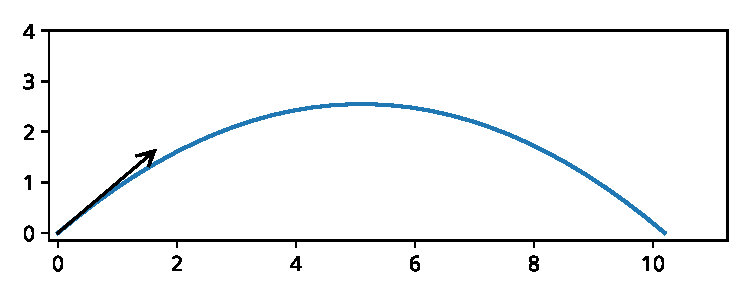
\includegraphics[width=0.99\linewidth]{figures/cannonball}
 \end{figure}
 \end{center}
 \vspace*{-2em}

\begin{center}
\begin{equation*}
x_{\text{final}} = f(\theta, v_0)
\end{equation*}
\end{center}
\end{frame}

\begin{frame}[fragile]{Cannonball}
\vspace*{-1em}
\begin{center}
 \begin{figure}
    	\centering
    	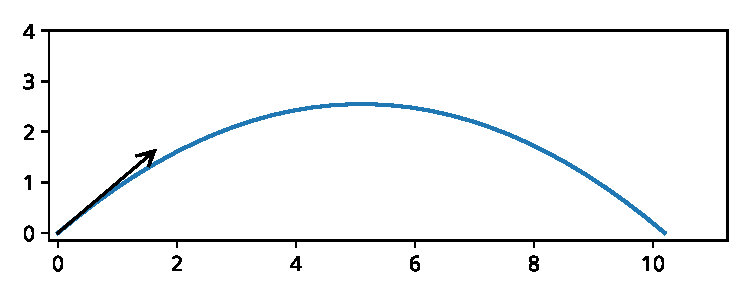
\includegraphics[width=0.99\linewidth]{figures/cannonball}
 \end{figure}
 \end{center}
 \vspace*{-2em}

\begin{center}
\begin{minted}[fontsize=\footnotesize]{python3} 
angle = np.deg2rad(45)
velocity = 10
g = 9.81
time_in_flight = 2 * velocity * np.sin(angle) / g
x = lambda t: velocity * np.cos(angle) * t
y = lambda t: velocity * np.sin(angle) * t - g * t**2 / 2
\end{minted}
\end{center}
\end{frame}

\begin{frame}[fragile]{Cannonball}
\vspace*{-1em}
\begin{center}
 \begin{figure}
    	\centering
    	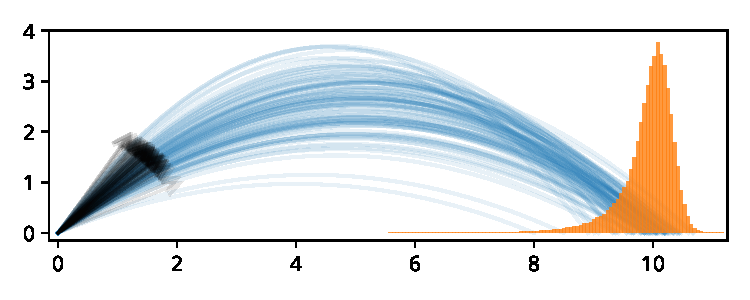
\includegraphics[width=0.99\linewidth]{figures/cannonball_sim1}
 \end{figure}
 \end{center}
 \vspace*{-2em}

\begin{center}
\begin{minted}[fontsize=\footnotesize]{python3} 
angle = np.deg2rad(random.gauss(45, 0.15 * 45)) # 15 % relative error
velocity = random.gauss(10, 0.01 * 10)          # 1 % relative error

# This is a nasty, non-linear function of velocity and angle
final_x = 2 * velocity**2 * np.cos(angle) * np.sin(angle) / g
\end{minted}
\end{center}
\end{frame}

\begin{frame}[fragile]{Mutual fund}
\begin{columns}
\begin{column}{0.55\textwidth}
    \begin{center}
    \vspace*{-4em}
	\begin{equation*}
	\textbf{money} = f(\text{yearly}, \text{interest\_rate})
	\end{equation*}
     \end{center}
\end{column}
\begin{column}{0.45\textwidth}  %%<--- here
    \begin{center}
     \begin{figure}
     	\centering
     	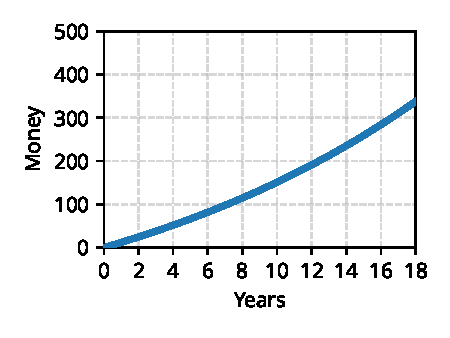
\includegraphics[width=0.99\linewidth]{figures/mutual_fund}
     \end{figure}
     \end{center}
\end{column}
\end{columns}
\end{frame}

\begin{frame}[fragile]{Mutual fund}
\begin{columns}
\begin{column}{0.55\textwidth}
    \begin{center}
     \begin{minted}[fontsize=\footnotesize]{python3} 


def simulate(years, yearly, interest):
    saved = 0
    yield saved
    for year in range(years):
        saved = saved * interest + yearly
        yield saved
        
years = 18
yearly = 12
interest = 1.05

list(simulate(years, yearly, interest))
     \end{minted}
     \end{center}
\end{column}
\begin{column}{0.45\textwidth}  %%<--- here
    \begin{center}
     \begin{figure}
     	\centering
     	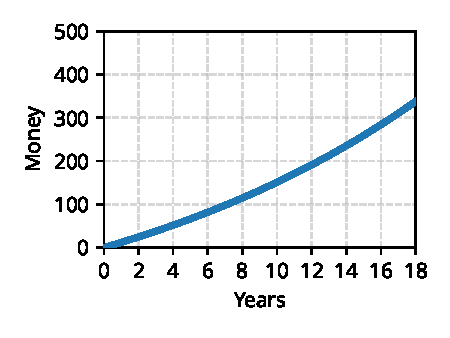
\includegraphics[width=0.99\linewidth]{figures/mutual_fund}
     \end{figure}
     \end{center}
\end{column}
\end{columns}
\end{frame}

\begin{frame}[fragile]{Mutual fund}
% comment: here we can ask interesting questions:
% - what is the probability of hitting 100 before x years?
% - after 5 years, what is the probability of hitting >= y?
\begin{columns}
\begin{column}{0.55\textwidth}
    \begin{center}
     \begin{minted}[fontsize=\footnotesize]{python3} 
import random

def simulate_rng(years, yearly, interest):
    saved = 0
    yield saved
    for year in range(years):
        ir = random.gauss(*interest)
        saved = saved * ir + yearly
        yield saved
        
years = 18
yearly = 12
interest = (1.05, 0.1)

list(simulate_rng(years, yearly, interest))
     \end{minted}
     \end{center}
\end{column}
\begin{column}{0.45\textwidth}  %%<--- here
    \begin{center}
     \begin{figure}
     	\centering
     	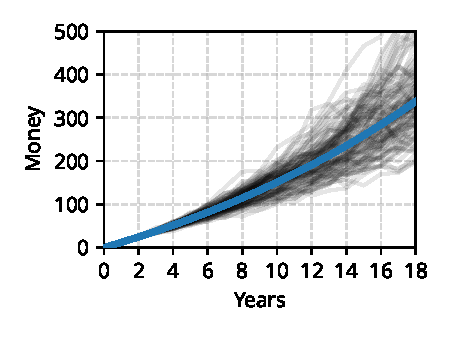
\includegraphics[width=0.99\linewidth]{figures/mutual_fund_simulations}
     \end{figure}
     \end{center}
\end{column}
\end{columns}
\end{frame}


\begin{frame}[fragile]{Monte Carlo Simulation}
	
	\begin{easylist}[itemize]
		# Uses uncertainty in inputs $\mathbf{x}$ to study uncertainty in $f(\mathbf{x})$
		# Draw many random realization of $\mathbf{x}$ and examine the outputs
		# Given $f$, it requires little math and is easy to program
		# Beware:
		## It can be hard to create distributions for $\mathbf{x}$
		## Sometimes $f$ is time consuming to compute
	\end{easylist}
\end{frame}

% ==================================================================
% ==================================================================
% ==================================================================
\section{Resampling}

\begin{frame}[fragile]{Resampling in code}
\begin{center}
\begin{minted}[fontsize=\footnotesize]{pycon} 
>>> import numpy as np
>>> elements = [1, 2, 3, 4, 5]

>>> np.random.choice(elements, replace=False, size=5) # Permutation
array([2, 4, 1, 5, 3])

>>> np.random.choice(elements, replace=True, size=5) # Resampling
array([4, 1, 1, 1, 1])

>>> p = [0.1, 0.1, 0.2, 0.3, 0.3] # With probabilities (weights)
>>> np.random.choice(elements, replace=False, size=3, p=p)
array([4, 5, 3])

>>> np.random.choice(elements, replace=True, size=3, p=p)
array([5, 5, 2])
\end{minted}
\end{center}
\end{frame}

\begin{frame}[fragile]{Height and pulse}
\begin{center}
 \begin{figure}
    	\centering
    	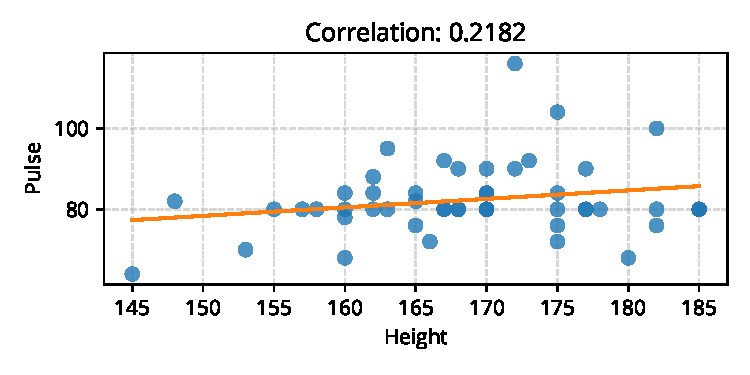
\includegraphics[width=0.99\linewidth]{figures/height_pulse_base.pdf}
 \end{figure}
 Is this a statistically significant correlation?\footnote{Dataset from \href{https://github.com/JedStephens/Handbook-of-Small-Data-Sets}{Handbook-of-Small-Data-Sets}}
 \end{center}
\end{frame}

\begin{frame}[fragile]{Height and pulse}
\begin{center}
 \begin{figure}
    	\centering
    	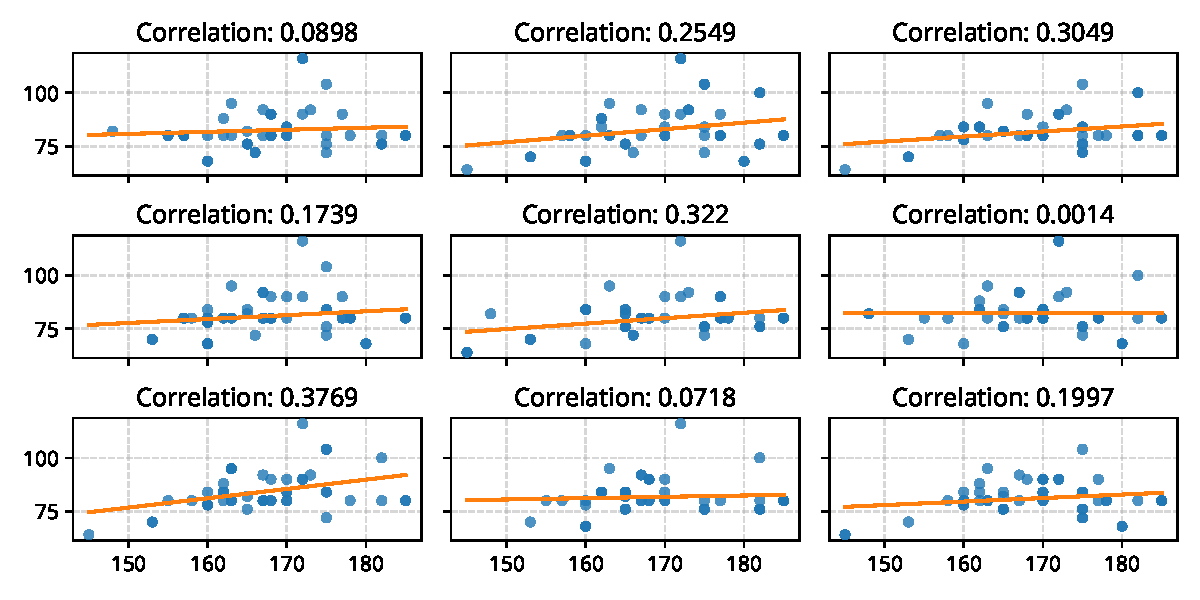
\includegraphics[width=0.99\linewidth]{figures/height_pulse_resamples.pdf}
 \end{figure}
 We sample the dataset by drawing pairs with replacement.
 \end{center}
\end{frame}


\begin{frame}[fragile]{Height and pulse}
\begin{center}
 \begin{figure}
    	\centering
    	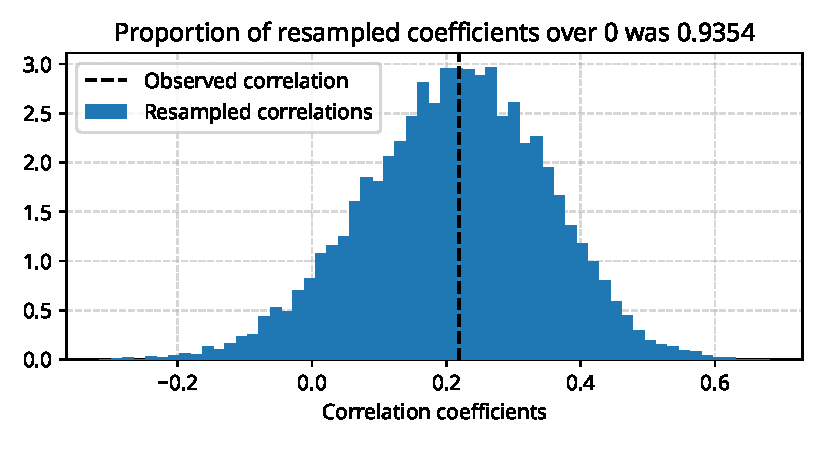
\includegraphics[width=0.99\linewidth]{figures/height_pulse_coefs_binned.pdf}
 \end{figure}
 Plot the distribution of resampled correlation coefficients.
 \end{center}
\end{frame}


\begin{frame}[fragile]{Groceries}
\begin{columns}
\begin{column}{0.50\textwidth}
    \begin{center}
     \begin{minted}[fontsize=\footnotesize]{pycon} 
>>> money_per_day
array([0, 0, 471.9, 784.22,0,  ...])
>>> money_per_day.sum()
8911.18
     \end{minted}
     \vspace*{2em}
     How much do I spend on\\groceries per month?
     \end{center}	
\end{column}
\begin{column}{0.50\textwidth}  %%<--- here
    \begin{center}
     \begin{figure}
     	\centering
     	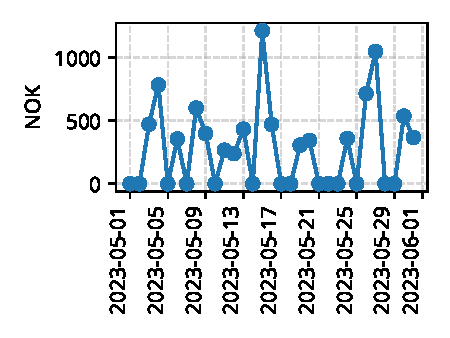
\includegraphics[width=0.99\linewidth]{figures/groceries_data}
     \end{figure}
     \end{center}
\end{column}
\end{columns}
\end{frame}

\begin{frame}[fragile]{Groceries}
\begin{center}
 \begin{figure}
    	\centering
    	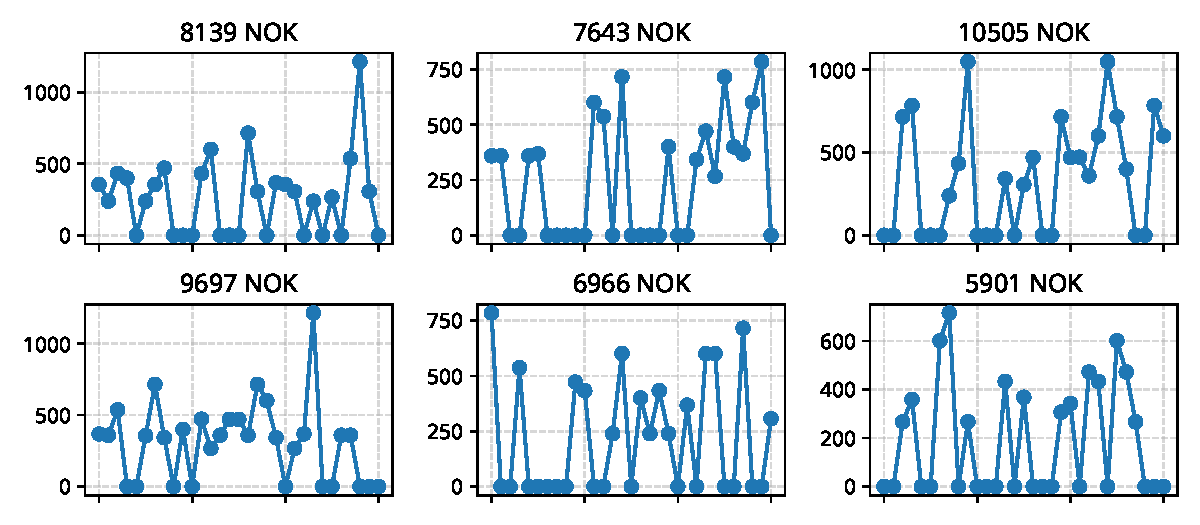
\includegraphics[width=0.99\linewidth]{figures/groceries_data_resamples}
 \end{figure}
 \end{center}

\begin{center}
\begin{minted}[fontsize=\footnotesize]{python3} 
import numpy as np

resamples = np.random.choice(money_per_day, 
            size=(9999, len(money_per_day)), 
            replace=True)
\end{minted}
\end{center}
     
\end{frame}

\begin{frame}[fragile]{Groceries}
\begin{center}
 \begin{figure}
    	\centering
    	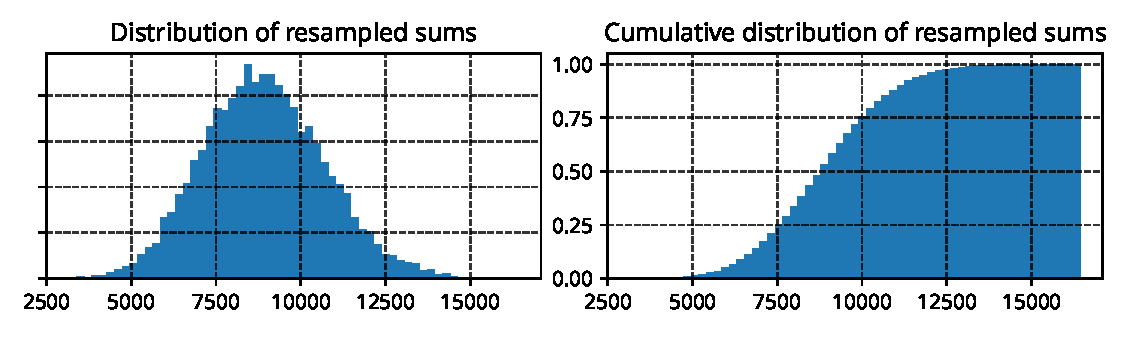
\includegraphics[width=0.99\linewidth]{figures/groceries_data_resampled}
 \end{figure}
 \end{center}

\begin{center}
\begin{minted}[fontsize=\footnotesize]{python3} 
import numpy as np
import matplotlib.pyplot as plt

resamples = np.random.choice(money_per_day, 
            size=(9999, len(money_per_day)), 
            replace=True)

plt.hist(resamples.sum(axis=1), bins="auto", 
         density=True, cumulative=True)
\end{minted}
\end{center}
\end{frame}

\begin{frame}[fragile]{Mutual fund}
 \begin{figure}
    	\centering
    	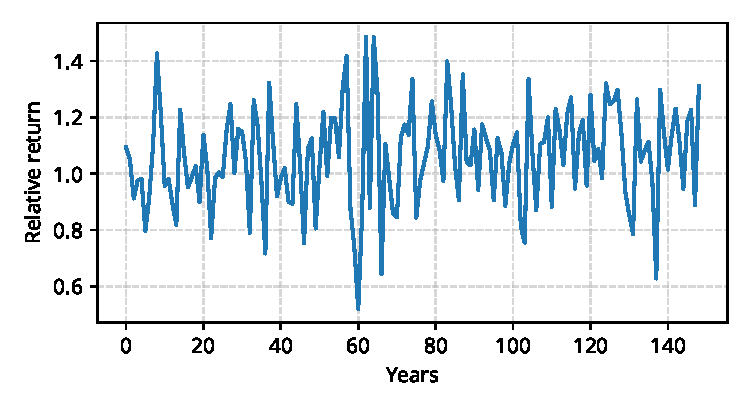
\includegraphics[width=0.99\linewidth]{figures/stock_returns}
 \end{figure}
\end{frame}

\begin{frame}[fragile]{Mutual fund}
 \begin{figure}
    	\centering
    	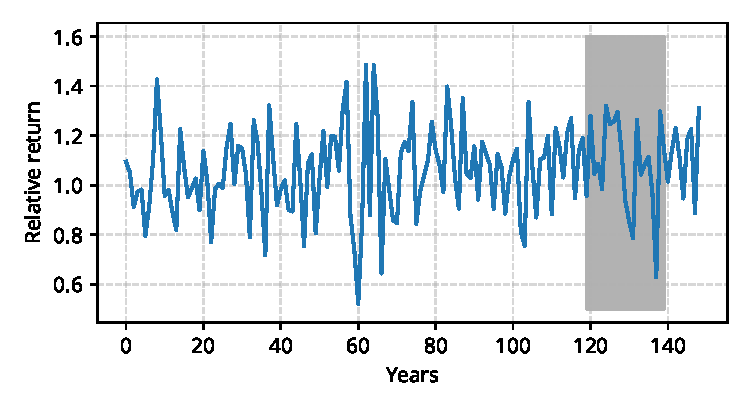
\includegraphics[width=0.99\linewidth]{figures/stock_returns_0}
 \end{figure}
\end{frame}

\begin{frame}[fragile]{Mutual fund}
 \begin{figure}
    	\centering
    	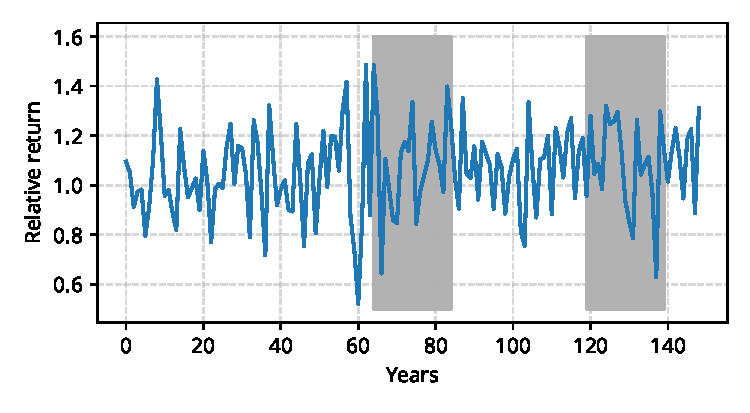
\includegraphics[width=0.99\linewidth]{figures/stock_returns_1}
 \end{figure}
\end{frame}

\begin{frame}[fragile]{Mutual fund}
 \begin{figure}
    	\centering
    	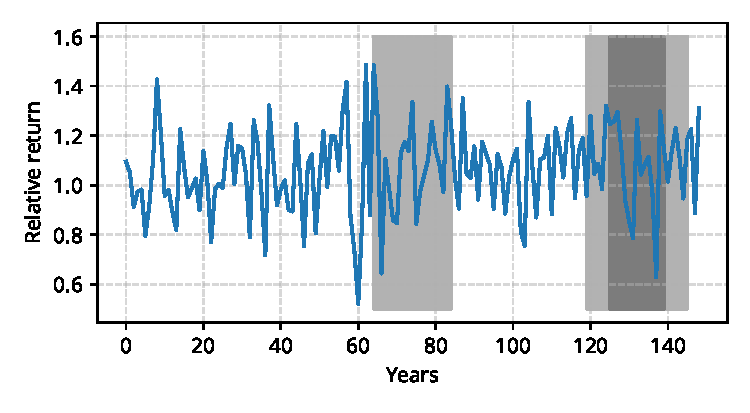
\includegraphics[width=0.99\linewidth]{figures/stock_returns_2}
 \end{figure}
\end{frame}



\begin{frame}[fragile]{Resampling}
	
	\begin{easylist}[itemize]
		# Often called \emph{bootstrapping}
		# Resampling with replacement gives estimates of uncertainty
		## The mean, the median, \textbf{the sum}, the standard deviation, \textbf{the correlation}, the difference between two groups
		# Beware
		## Sample size should not be too small
		## Distributional assumptions can be a better choice
	\end{easylist}
\end{frame}


% ==================================================================
% ==================================================================
% ==================================================================
\section{Stochastic search}

\begin{frame}[fragile]{Wind farm layout optimization}
\vspace*{-1em}
\begin{center}
 \begin{figure}
    	\centering
    	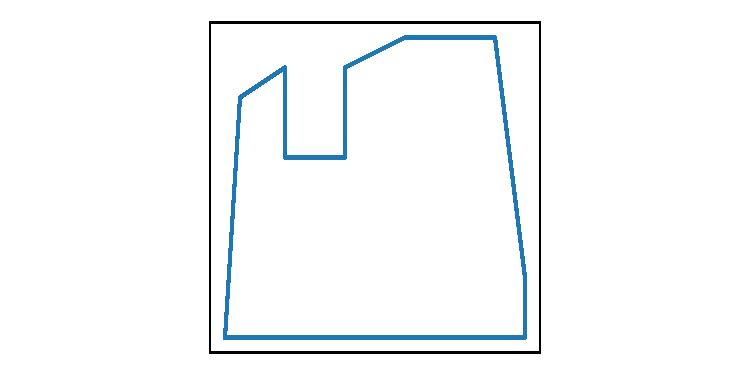
\includegraphics[width=0.99\linewidth]{figures/windfarm}
 \end{figure}
 \end{center}
\vspace*{-2em}
\begin{center}
Place 25 wind turbine on the acreage, so as to\\
(1) maximize distance to closest neighboring wind turbine \\
(2) minimize distance to acreage area border (if outside)
\end{center}
\end{frame}

\begin{frame}[fragile]{Wind farm layout optimization}
\vspace*{-1em}
\begin{center}
 \begin{figure}
    	\centering
    	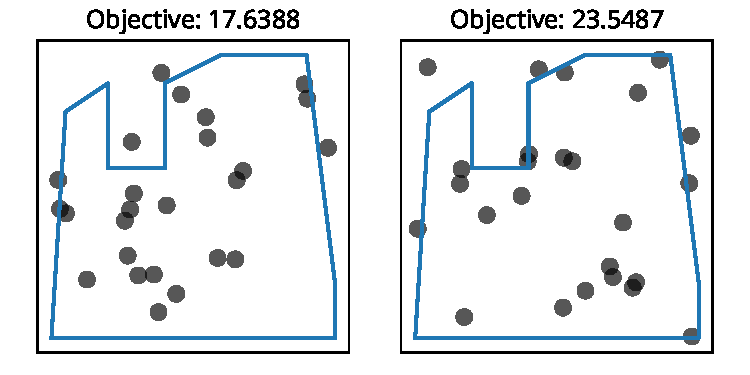
\includegraphics[width=0.99\linewidth]{figures/windfarm_random_solution}
 \end{figure}
 \end{center}
\vspace*{-2em}
\begin{center}
\begin{minted}[fontsize=\small]{pycon}
>>> points = np.random.uniform(size=(25, 2))
>>> objective(points)
17.6388238637308
\end{minted}
\end{center}
\end{frame}

\begin{frame}[fragile]{Wind farm layout optimization - hill climbing}
\vspace*{-1em}
\begin{center}
 \begin{figure}
    	\centering
    	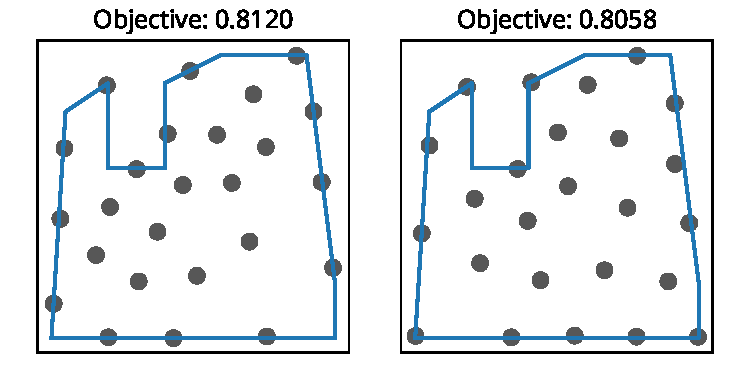
\includegraphics[width=0.99\linewidth]{figures/windfarm_hc}
 \end{figure}
 \end{center}
\vspace*{-2em}
\begin{center}
\begin{minted}[fontsize=\footnotesize]{pycon}
>>> idx = np.random.choice(np.arange(points.shape[0]))
>>> points[idx, :] += np.random.normal(loc=0, scale=0.05, size=(2))
\end{minted}
\end{center}
\end{frame}

\begin{frame}[fragile]{Wind farm layout optimization - annealing}
\vspace*{-1em}
\begin{center}
 \begin{figure}
    	\centering
    	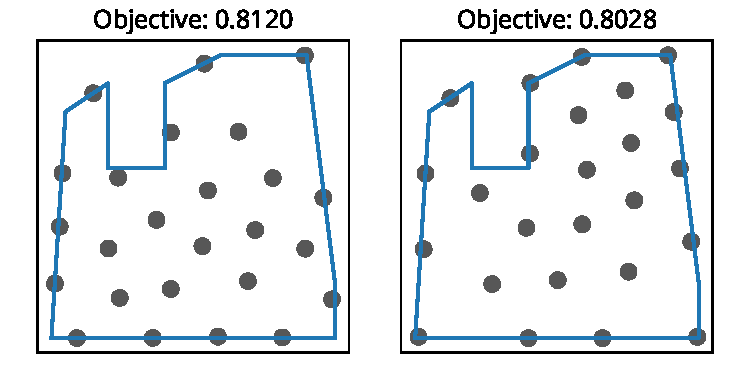
\includegraphics[width=0.99\linewidth]{figures/windfarm_sa}
 \end{figure}
 \end{center}
\vspace*{-2em}
\begin{center}
\begin{minted}[fontsize=\footnotesize]{python3}
    suggestion = permute_solution(points)

    accept_worse = np.random.rand() < np.exp(-0.01 * iteration)
    if objective(suggestion) < objective(points) or accept_worse:
        points = suggestion
\end{minted}
\end{center}
\end{frame}


\begin{frame}[fragile]{Pupil-classroom assignments}
\vspace*{-1em}
\begin{center}
Pupils are to be allocated to classrooms\\
Each pupil writes a list with their top-$3$ desired classmates \\
\vspace*{2em} 
Place 100 pupils in 5 groups of 20, so that \\
(1) the average pupil is as happy as possible and \\
(2) the least happy pupil is as happy as possible
\vspace*{1em} 
\begin{equation*}
\binom{100}{20}
\binom{80}{20}
\binom{60}{20}
\binom{40}{20}
\binom{20}{20}
\frac{1}{5!} \approx 4.496 \times 10^{18}
\end{equation*}
\end{center}
\end{frame}

\begin{frame}[fragile]{Pupil-classroom assignments}
\vspace*{-1.5em}
\begin{center}
 \begin{figure}
    	\centering
    	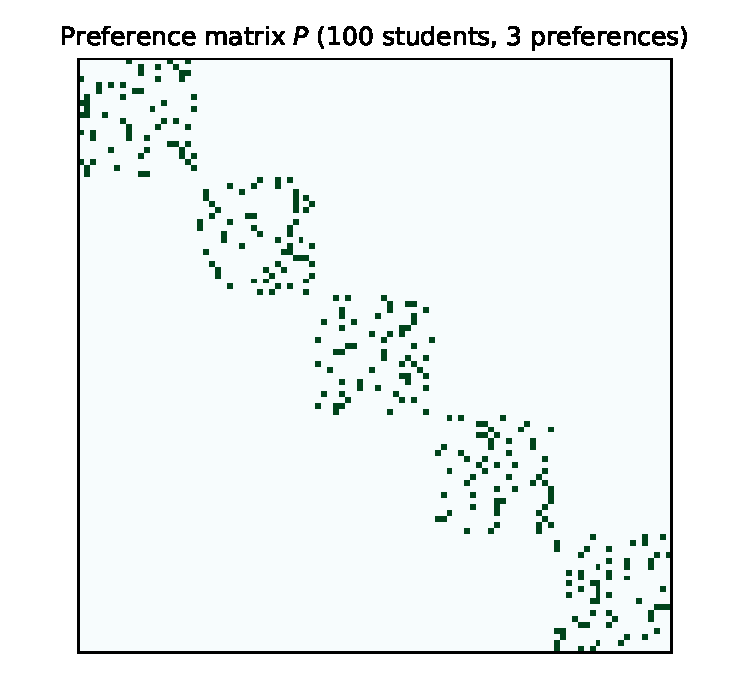
\includegraphics[width=0.6\linewidth]{figures/classroom_matrix_structures.pdf}
 \end{figure}
 \end{center}
\vspace*{-2em}
\begin{center}
Here's a problem instance with a known best solution
\end{center}
\end{frame}

\begin{frame}[fragile]{Pupil-classroom assignments}
\vspace*{-1.5em}
\begin{center}
 \begin{figure}
    	\centering
    	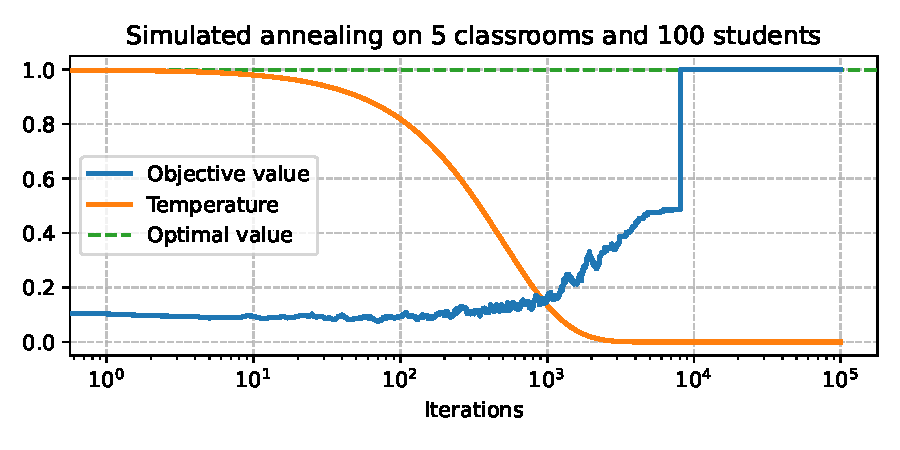
\includegraphics[width=0.99\linewidth]{figures/classroom_sim_annealing.pdf}
 \end{figure}
 \end{center}
\vspace*{-2em}
\begin{center}
Swap two pupils at random, then re-evaluate
\end{center}
\end{frame}

\begin{frame}[fragile]{Pupil-classroom assignments}
\vspace*{-1.5em}
\begin{center}
 \begin{figure}
    	\centering
    	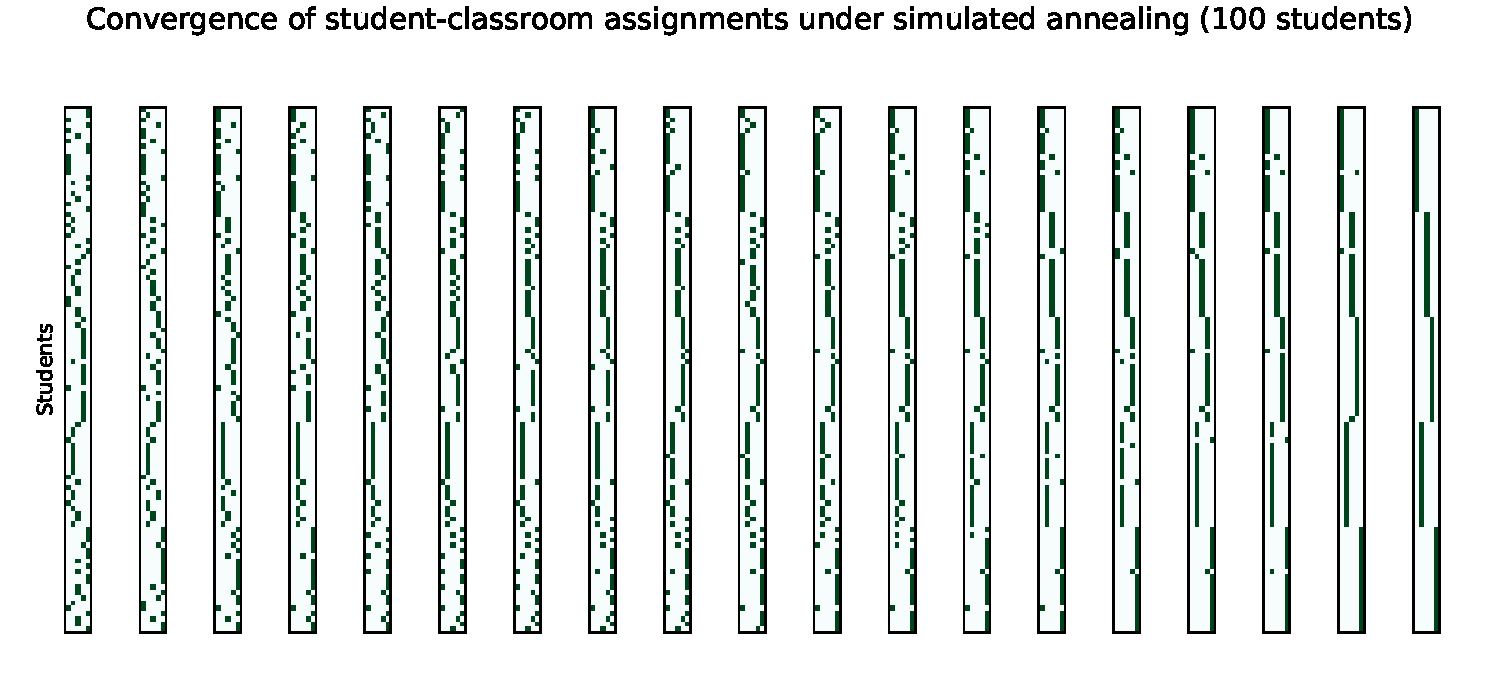
\includegraphics[width=0.99\linewidth]{figures/classroom_convergence.pdf}
 \end{figure}
 \end{center}
\vspace*{-2em}
\begin{center}
Problem solved to optimality in $\sim 1$ second
\end{center}
\end{frame}


\begin{frame}[fragile]{Stochastic search}
	\begin{easylist}[itemize]
		# Good for combinatorial problems with non-linear objectives
		# In its simplest form: try, evaluate, try again
		## More advanced: simulated annealing
		% # Constraints may be softened and put into the objective
		# You need: 
		## a way to generate/modify solutions
		## an objective to evaluate
		# Beware:
		## If the objective has simple form, exploit it (MIP)
		## No guarantees of optimal solution, it's a heuristic only
		## Typically poor performance on contrained problems
	\end{easylist}
\end{frame}




% ==================================================================
% ==================================================================
% ==================================================================
\section{Inverse probability (Bayesian statistics)}

\begin{frame}[fragile]{Inverse problems}
\begin{columns}
\begin{column}{0.5\textwidth}
    \begin{center}
\textbf{Deterministic}\\
\vspace*{2em}
\textbf{Forward (simulation)} \\
Given input x,\\determine the output f(x) \\
\vspace*{1em}
\textbf{Backward (optimization)} \\
Given output y = f(x),\\find the input x
     \end{center}
\end{column}
\begin{column}{0.5\textwidth}  %%<--- here
    \begin{center}
\textbf{Stochastic}\\
\vspace*{2em}
\textbf{Foward (Monte Carlo)} \\
Given a distribution over x,\\find the distribution f(x) \\
\vspace*{1em}
\textbf{Backward (Bayes)} \\
Given a distribution y = f(x),\\find the distribution of input x
     \end{center}
\end{column}
\end{columns}
\end{frame}


\begin{frame}[fragile]{Mutual fund revisited}
\vspace*{-1em}
\begin{center}
 \begin{figure}
    	\centering
    	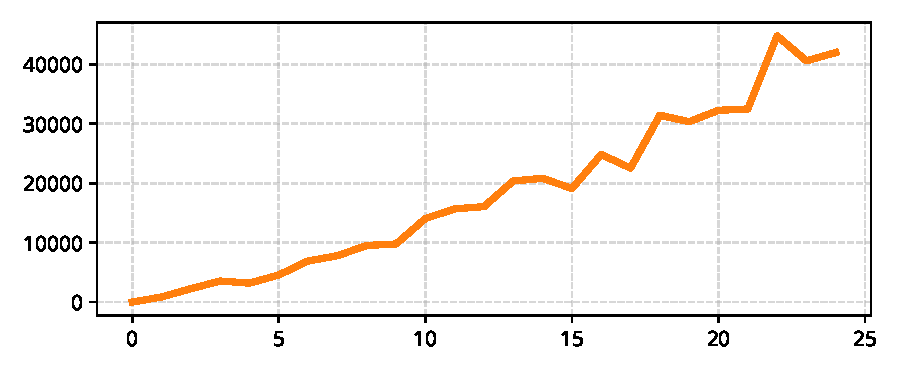
\includegraphics[width=0.9\linewidth]{figures/esmda_observations.pdf}
 \end{figure}
 Given a prior $p(x)$ on parameters $x$ and a likelihood $p(y \mid x)$, \\
 we wish to find $p(x \mid y) \propto p(y \mid x) p(x)$.
 \end{center}
\end{frame}

\begin{frame}[fragile]{Mutual fund revisited}
\vspace*{-1em}
\begin{center}
 \begin{figure}
    	\centering
    	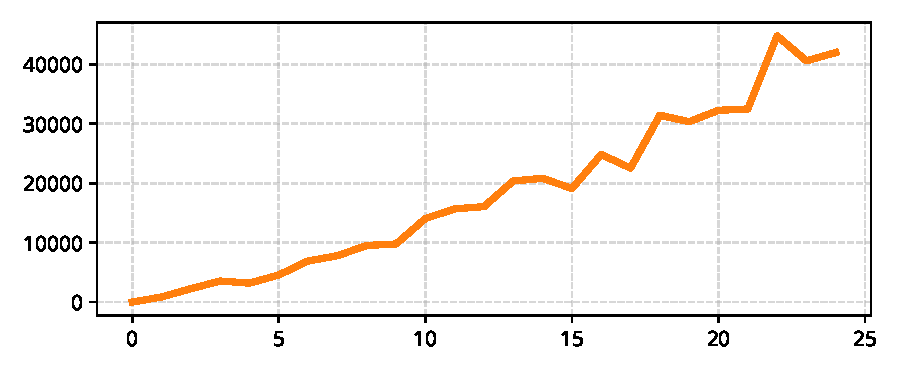
\includegraphics[width=0.9\linewidth]{figures/esmda_observations.pdf}
 \end{figure}
 \begin{center}
 Ensemble Smoother - Multiple Data Assimilation
 \end{center}
\begin{align*}
\log p(x \mid y) 
&\propto \log p(y \mid x) + \log p(x) \\
&\propto
\underbrace{(g(x) - d)^T C_D^{-1} (g(x) - d)}_{\text{distance from observed values}} +
\underbrace{(x - \mu)^T C_M^{-1} (x - \mu) }_{\text{distance from prior}}
\end{align*}
 \end{center}
\end{frame}

\begin{frame}[fragile]{Mutual fund revisited}
\vspace*{-1em}
\begin{center}
 \begin{figure}
    	\centering
    	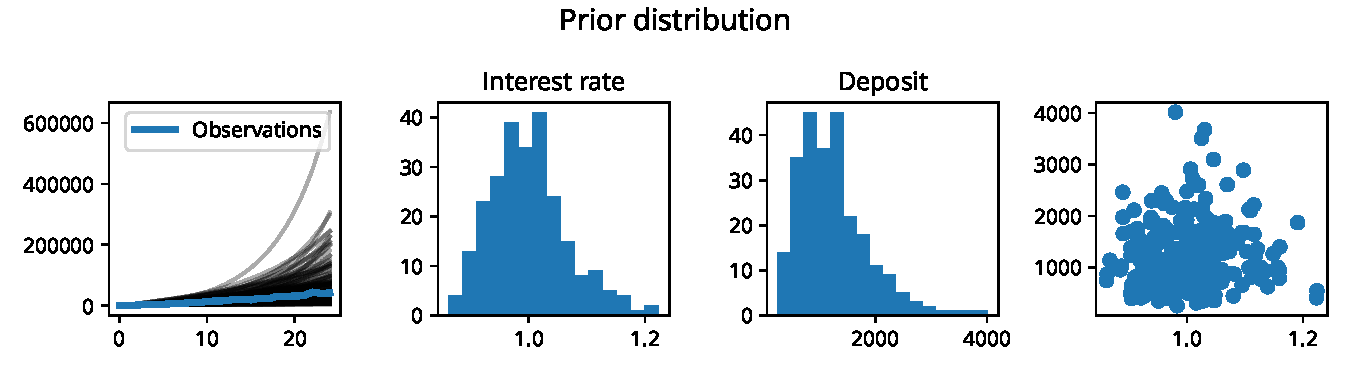
\includegraphics[width=0.99\linewidth]{figures/esmda_prior_no_truth.pdf}
 \end{figure}
 Here we see a prior $p(x)$ on parameters ``interest rate'' and ``deposit.''\footnote{We'll use ESMDA from the Equinor repository\\ \href{https://github.com/equinor/iterative_ensemble_smoother}{https://github.com/equinor/iterative\_ensemble\_smoother}}
 \end{center}
\end{frame}

\begin{frame}[fragile]{Mutual fund revisited}
\vspace*{-1em}
\begin{center}
 \begin{figure}
    	\centering
    	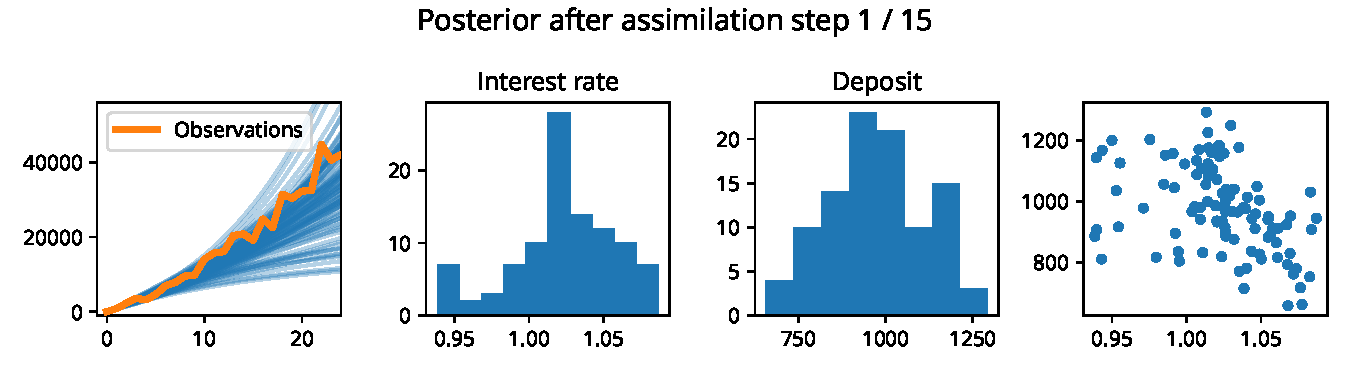
\includegraphics[width=0.99\linewidth]{figures/esmda_step_1.pdf}
 \end{figure}
  Running data assimilation iterations ...
 \end{center}
\end{frame}

\begin{frame}[fragile]{Mutual fund revisited}
\vspace*{-1em}
\begin{center}
 \begin{figure}
    	\centering
    	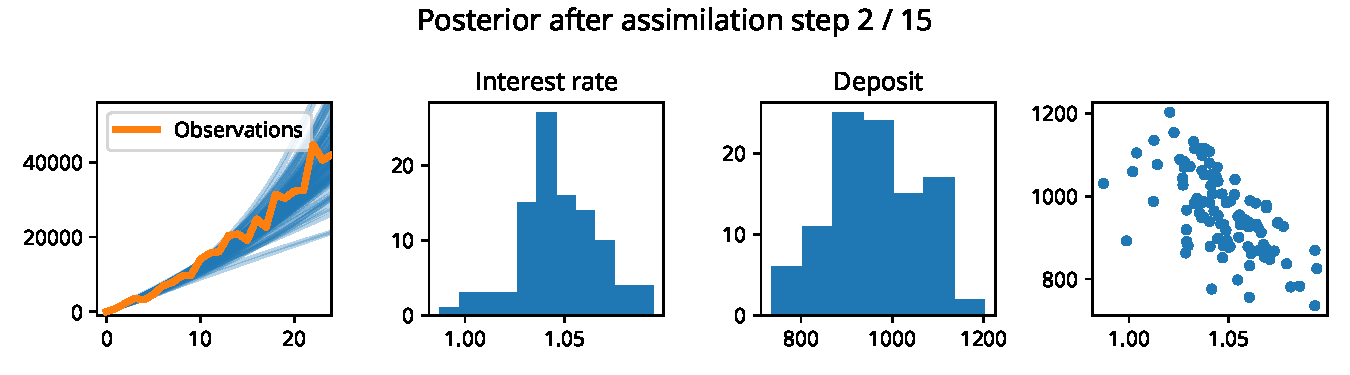
\includegraphics[width=0.99\linewidth]{figures/esmda_step_2.pdf}
 \end{figure}
   Running data assimilation iterations ...
 \end{center}
\end{frame}

\begin{frame}[fragile]{Mutual fund revisited}
\vspace*{-1em}
\begin{center}
 \begin{figure}
    	\centering
    	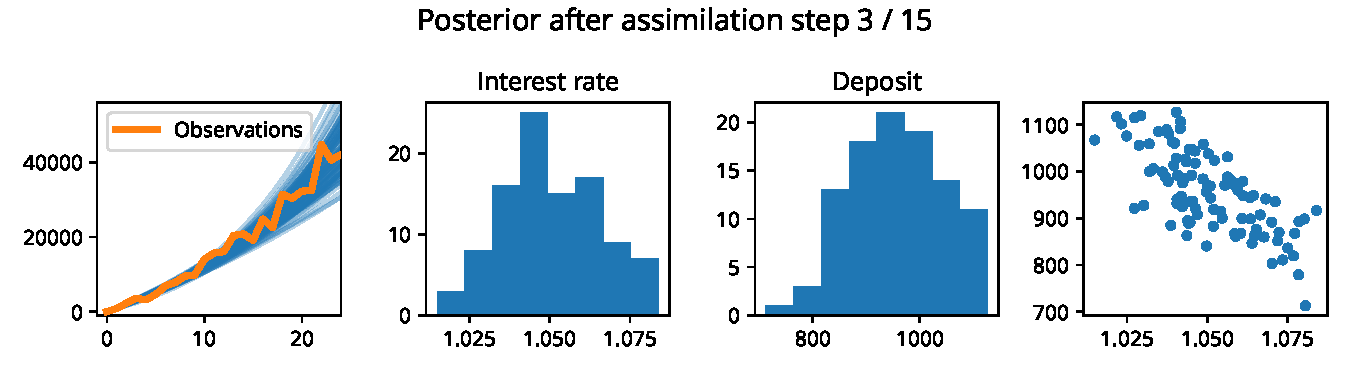
\includegraphics[width=0.99\linewidth]{figures/esmda_step_3.pdf}
 \end{figure}
   Running data assimilation iterations ...
 \end{center}
\end{frame}

\begin{frame}[fragile]{Mutual fund revisited}
\vspace*{-1em}
\begin{center}
 \begin{figure}
    	\centering
    	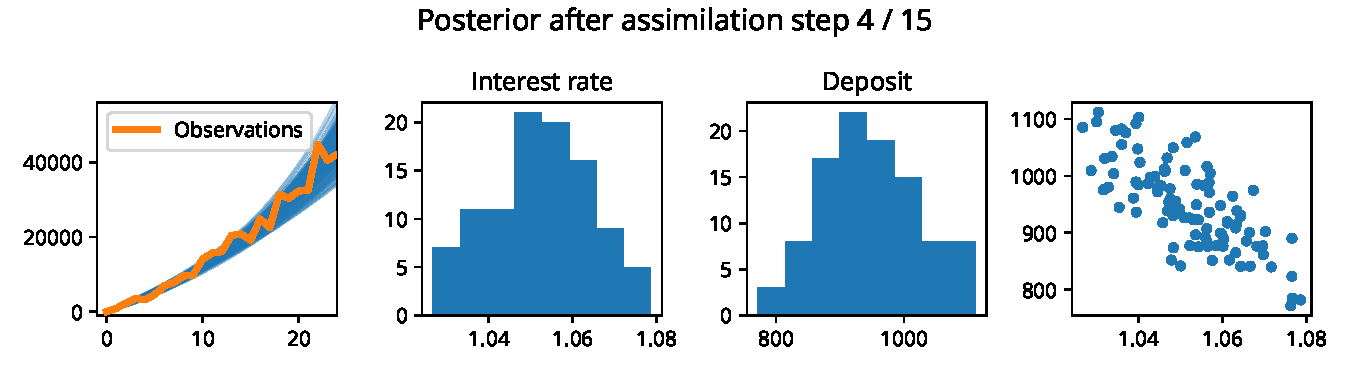
\includegraphics[width=0.99\linewidth]{figures/esmda_step_4.pdf}
 \end{figure}
   Running data assimilation iterations ...
 \end{center}
\end{frame}

\begin{frame}[fragile]{Mutual fund revisited}
\vspace*{-1em}
\begin{center}
 \begin{figure}
    	\centering
    	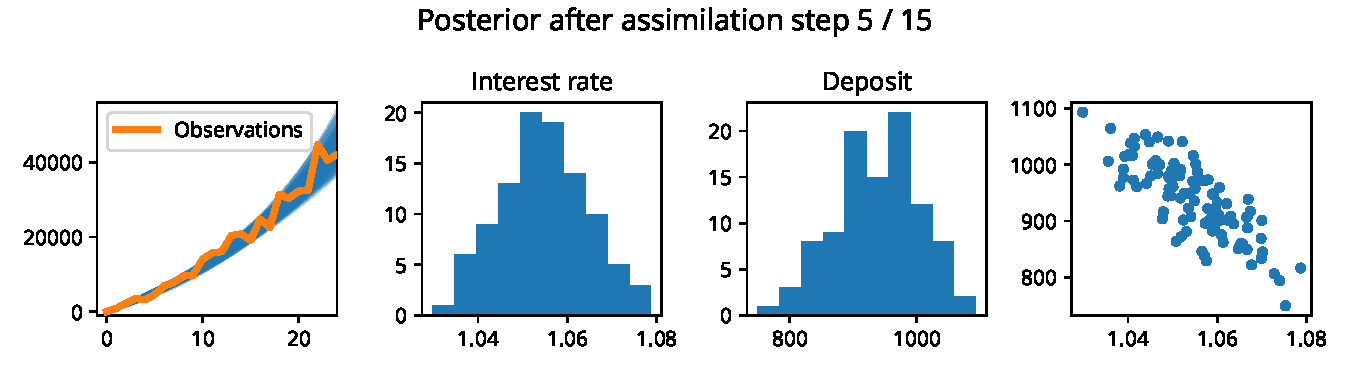
\includegraphics[width=0.99\linewidth]{figures/esmda_step_5.pdf}
 \end{figure}
   Running data assimilation iterations ...
 \end{center}
\end{frame}

\begin{frame}[fragile]{Mutual fund revisited}
\vspace*{-1em}
\begin{center}
 \begin{figure}
    	\centering
    	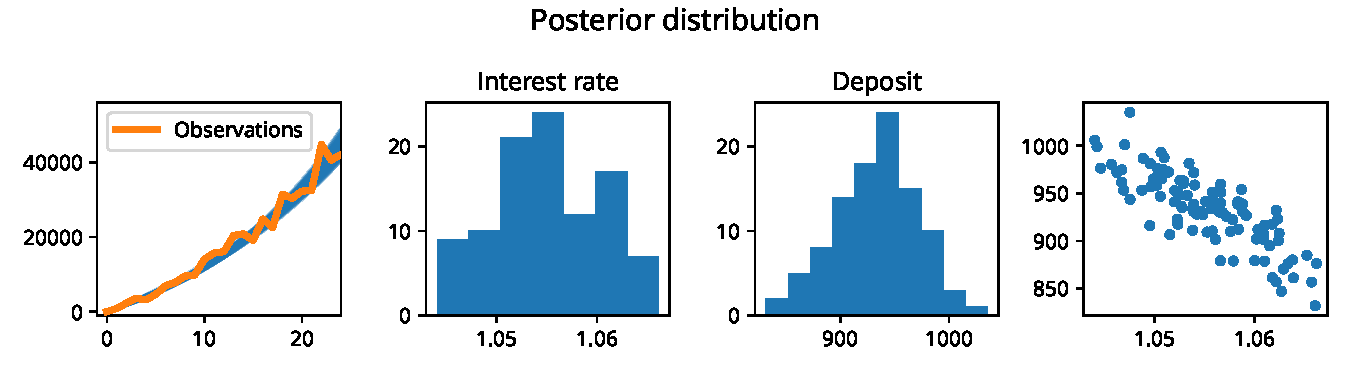
\includegraphics[width=0.99\linewidth]{figures/esmda_posterior_no_truth.pdf}
 \end{figure}
 We now have samples from $p(x \mid y)$\\ \vspace*{1em}
 A balance of (1) respecting the prior \\and (2) matching the observations
 \end{center}
\end{frame}


\begin{frame}[fragile]{Inverse probability (Bayesian statistics)}
	\begin{easylist}[itemize]
		# Find the posterior distribution of parameters, given (1)
		a prior on the parameters and (2) and likelihood
		\begin{equation*}
		p(x \mid y) \propto p(y \mid x) p(x)
		\end{equation*}
		# Can be used with most models, e.g. linear regression
		# Excellent choice in \emph{small data problems}
		# Data assimilation performs very crude 
		bayesian inference, but is the only choice when the model is expensive to evaluate
	\end{easylist}
\end{frame}



\begin{frame}[fragile]{References and further reading}
\scriptsize
\begin{easylist}[itemize]
# Statistics
## Statistical Inference by Casella et al (2001).
## All of Statistics by Larry Wasserman (2010).
## Statistical Rethinking by Richard McElreath (2020).
# Optimization by search
## Artificial Intelligence: A Modern Approach by Norvig et al (2009).
## Essentials of Metaheuristics by Sean Luke (2012).
# Popular science
## The Visual Display of Quantitative Information by Edward R. Tufte (2001).
## Flaws and Fallacies in Statistical Thinking by Stephen K. Campbell (2012).
\end{easylist}
\normalsize
\begin{center}
Code for presentation and all figures: { \href{https://github.com/tommyod/rng}{https://github.com/tommyod/rng}}
\end{center}
\end{frame}

\end{document}
